\documentclass[12pt]{article}

\usepackage{graphicx}
\usepackage{amssymb}
\usepackage{gensymb}
\usepackage{bm}
\usepackage{hyperref}
\usepackage[utf8]{inputenc}

\begin{document}
\part{Aan/uit positiecontrole van een motor}
\section{Introductie}
Volgend systeem beschrijft een motor met aan/uit-regeling. Dit systeem bestaat uit een lineair en niet-lineair deel. De regelkring wordt weergegeven in figuur \ref{regellus}.
\begin{figure}[!h]
	\centering
	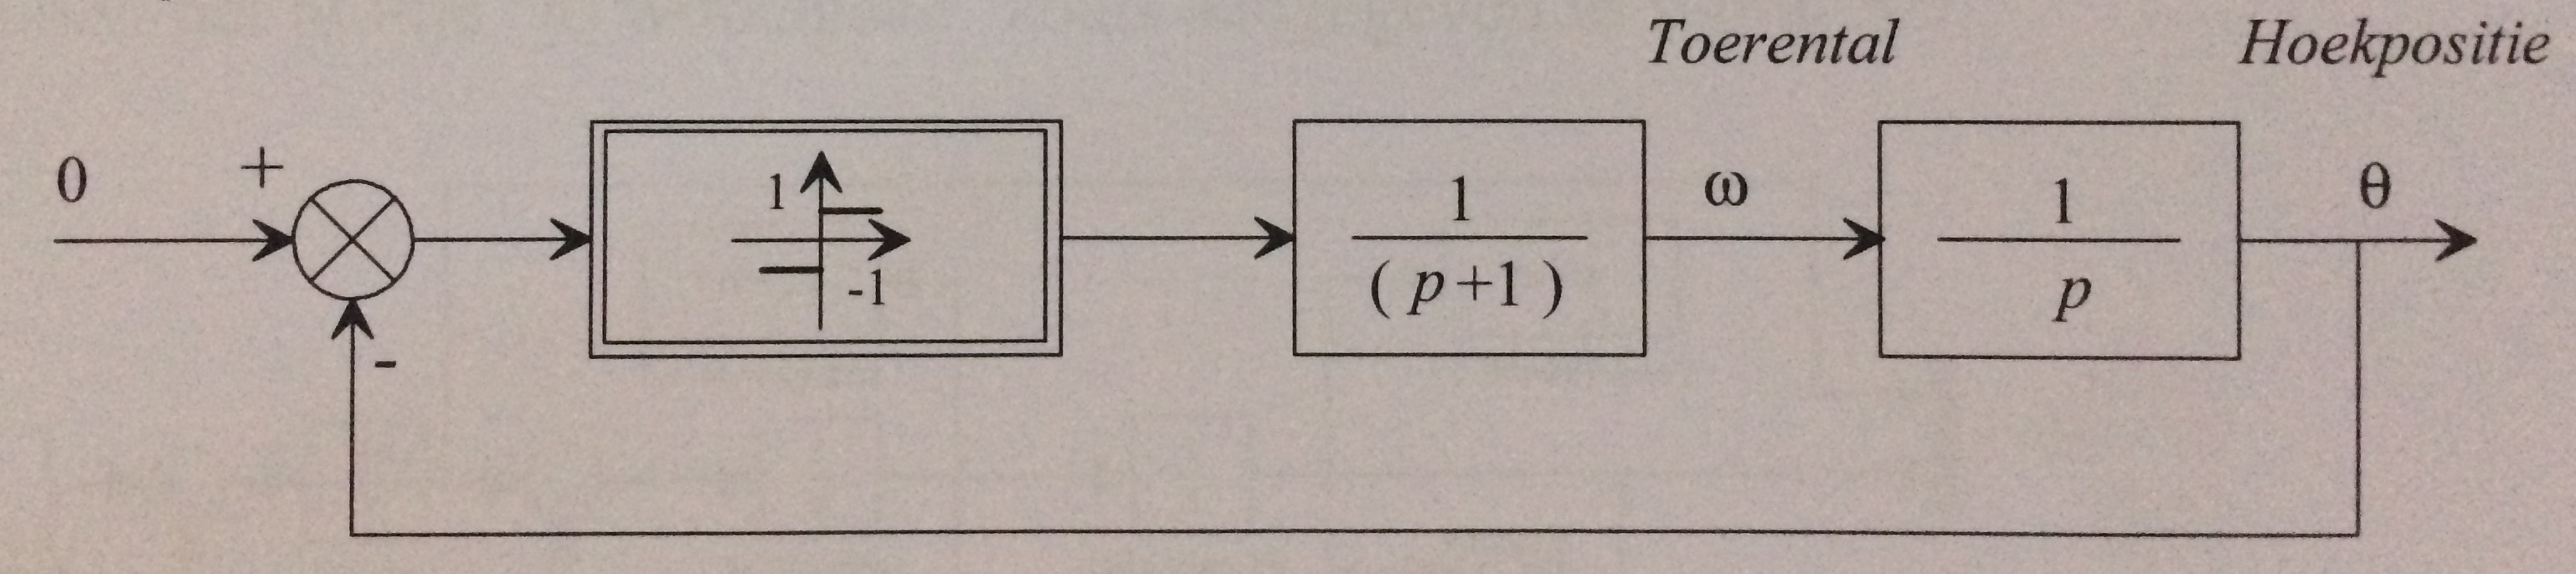
\includegraphics[width=\textwidth, keepaspectratio]{regellus.png}
	\caption{Regellus voor Aan/uit positieregeling}
	\label{regellus}	
\end{figure}
\noindent
Het niet-lineaire deel bestaat uit het aan/uit-element. Deze schakelt tussen de waarden +1 en -1 om de motor respectievelijk positief en negatief te laten draaien. De motor zelf is een eerste orde systeem met transfertfunctie $TF_{motor} = \frac{1}{p+1}$. Hieruit volgt dat $K=1$ en $\tau=1$. Gezien de hoekpositie graag gekend is wordt er tenslotte een zuivere integrator toegevoegd. Immers geldt dat $\theta = \int_{\Delta t} \omega \ \mathrm{d}t$. \\ \\
\section{Simulaties}
\subsection{Tijdsverloop en Fasetraject}
Om deze schakeling te simuleren in SIMULINK werd gebruik gemaakt van het schema uit figuur \ref{simulinkschema}. Deze omzetting maakt het mogelijk om de beginwaarden van $\omega$ en $\theta$ te kiezen. Als beginwaarden werden gekozen:
\[ 
\left \{
  \begin{tabular}{c}
  $\omega_0 = 2$ rad/s \\
  $\theta_0 = 1.5$ rad
  \end{tabular}
\right. 
\]
\begin{figure}
	\centering
	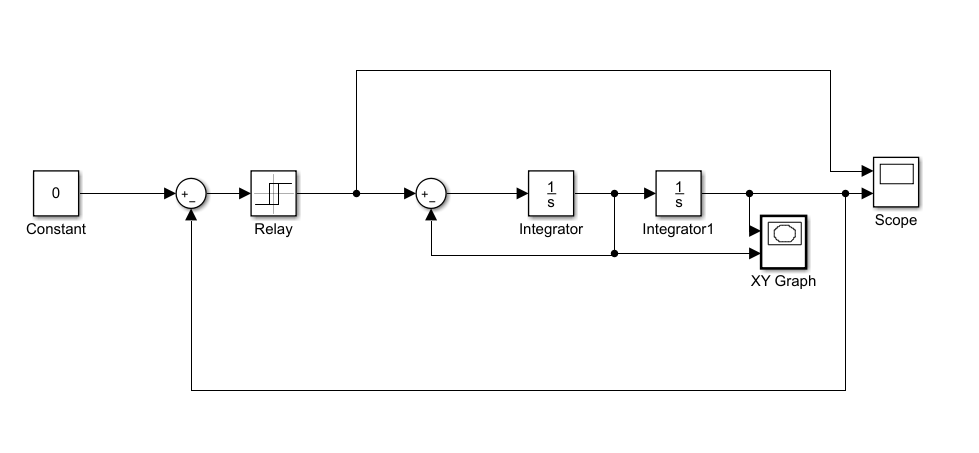
\includegraphics[width=\textwidth, keepaspectratio]{simulinkschema.png}
	\caption{Gesimuleerd schema in SIMULINK}
	\label{simulinkschema}
\end{figure}
Na een simulatie van 10 seconden levert dit de output uit figuur \ref{output1}.
\begin{figure}
	\centering
	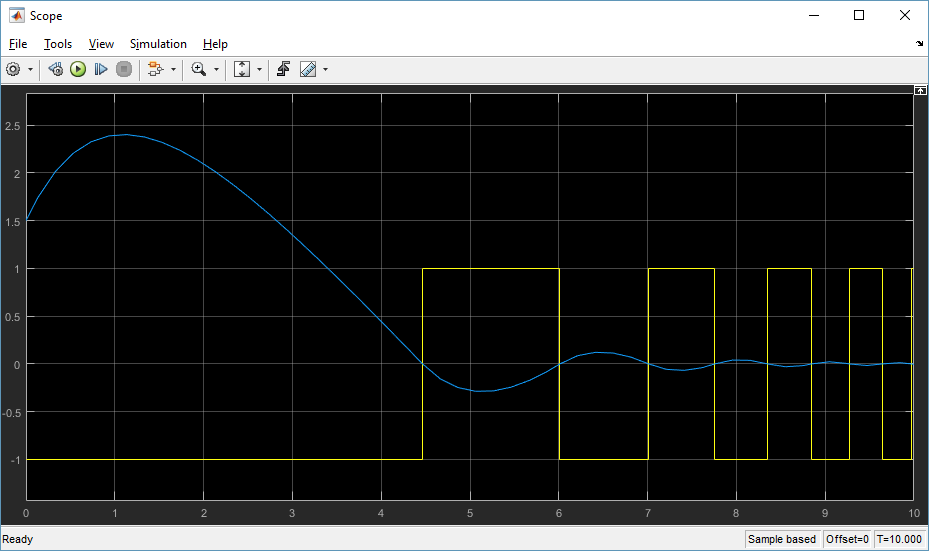
\includegraphics[width=\textwidth, keepaspectratio]{output1.png}
	\caption{Tijdsverloop (10 seconden) voor $\omega_0 = 2$ rad/s en $\theta_0 = 1.5$ rad (zonder hysteresis)}
	\label{output1}
\end{figure}
\noindent De fasetrajecten worden bepaald door $\omega$ uit te zetten als een functie van $\theta$. Deze waarden zijn rechtstreeks toegankelijk in het schema en worden geplot in een XY-grafiek. Dit levert het resultaat uit figuur \ref{xynohys}. Indien men het fasetraject wil bekomen met hysteresis dient het relais pas aan/uit te schakelen bij een bepaalde waarde. Voor figuur \ref{xyhys} werd een uit/aan-schakelwaarde van $[-0.5;0.5]$ gekozen. \\ \\
Het valt op dat de figuur met hysteresis blijkt te convergeren naar de waarde 0. Dit komt overeen met het gesimuleerde tijdsverloop uit figuur \ref{output1}. Hierin blijkt immers ook dat na een langere tijd de outputwaarde convergeert naar 0. Ook blijkt dat het schakelelement (gele lijn) frequenter zal aan/uit schakelen. Dit is ook logisch gezien de outputwaarde constant sneller door 0 zal gaan en de schakelaar dus vaker probeert het systeem te corrigeren. \\ \\
Voor het tijdsverloop van het systeem inclusief hysteresis te simuleren werd gebruik gemaakt van volgende waarden:
\[ 
\left \{
  \begin{tabular}{c}
  $\omega_0 = 0.75$ rad/s \\
  $\theta_0 = 1$ rad \\
  hysteresis = $\pm 0.4$
  \end{tabular}
\right. 
\]
Het fasetraject wordt afgebeeld in figuur \ref{xytwo}. Deze figuur komt overeen met de eerder geziene figuur voor hysteresis. Twee belangrijke verschillen zijn de volgende:
\begin{itemize}
	\item Het beginpunt ligt anders. Deze is afhankelijk van de gekozen beginwaarden. In dit geval ligt het beginpunt op $[1;0.75]$. 
	\item De breedte van de hysteresislus is verkleind. Dit valt te verklaren uit het kleiner gekozen hysteresinterval.
\end{itemize}
Het tijdsverloop wordt afgebeeld in figuur \ref{output2}. Hierin valt duidelijk de oscillatie te merken. Dit is te danken aan de ingesteld hysteresis. Bij $\theta = \pm 0.4$ zal het schakelelement omschakelen. Dit zorgt ervoor dat de motor zal omkeren. Hoewel deze output een grotere fout vertoont, is deze manier van regelen meer gewenst. In de eerdere figuur viel immers op hoe het schakelelement steeds frequenter begon te schakelen. Dit zorgt ervoor dat dit element sneller tot aan zijn maximale schakelfrequentie zal geraken, met stuk gaan tot gevolg. 
\newpage
\begin{figure}[!h]
	\centering
	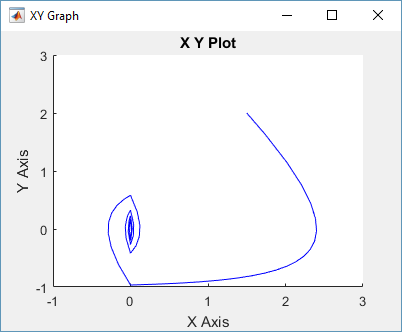
\includegraphics[height=0.4\textheight, keepaspectratio]{xynohys.png}
	\caption{Fasetraject (geen hysteresis)}
	\label{xynohys}
\end{figure}
\begin{figure}[!h]
	\centering
	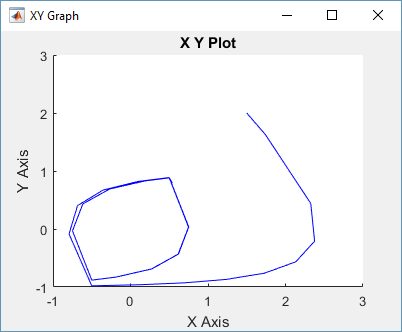
\includegraphics[height=0.4\textheight, keepaspectratio]{xyhys.png}
	\caption{Fasetraject (hysteresis)}
	\label{xyhys}
\end{figure}
\begin{figure}[!h]
	\centering
	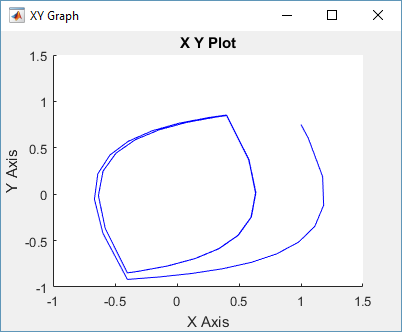
\includegraphics[height=0.4\textheight, keepaspectratio]{xytwo.png}
	\caption{Fasetraject voor $\omega_0 = 0.75$ rad/s en $\theta_0 = 1$ rad en hysteresis = $\pm 0.4$}
	\label{xytwo}
\end{figure}
\begin{figure}[]
	\centering
	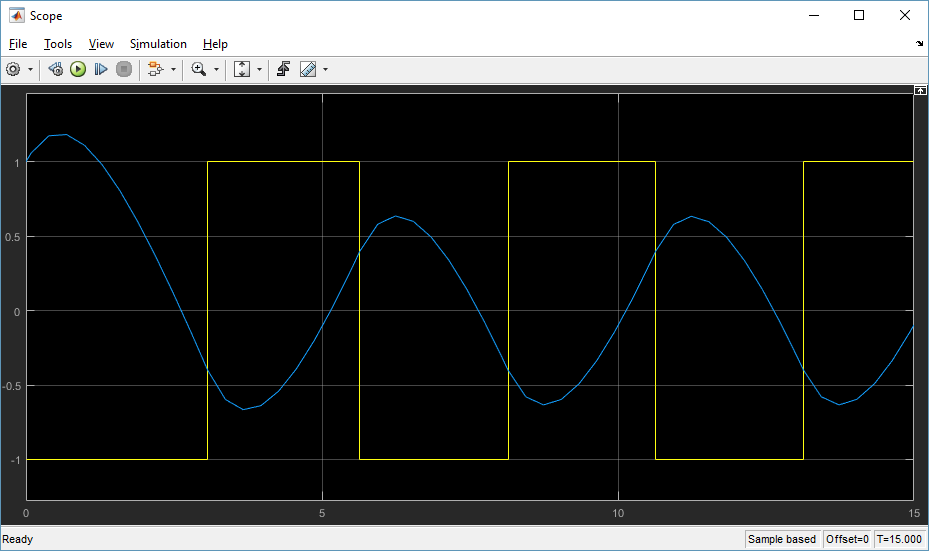
\includegraphics[width=\textwidth, keepaspectratio]{output2.png}
	\caption{Tijdsverloop (15 seconden) voor $\omega_0 = 0.75$ rad/s en $\theta_0 = 1$ rad en hysteresis = $\pm 4$)}
	\label{output2}
\end{figure}
\clearpage
\subsection{Hysteresisbreedte voor $t_{osc}$ = 2s}
Voor de hysteresisbreedte te bepalen bij een bepaalde oscillatietijd werd gebruik gemaakt van de beschrijvende-functiemethode. Voor een aan-uit regelaar met hysteresis geldt:
\begin{equation}
	N = \frac{4M}{\pi * E_m} * \mathrm{e}^{-j*\omega t}
\end{equation}
Herschreven zodat deze ook in functie staat van de hysteresisbreedte:
\begin{equation}
	N = \frac{4M}{\pi * E_m} * \mathrm{e}^{-j*\arcsin(\frac{D}{E_m})}
	\label{hbreedte}
\end{equation} 
Hierbij staat $M$ voor de amplitude van de hysteresislus, $D$ voor de hysteresisbreedte en $E_m$ voor de amplitude van het errorsignaal. \\ \\
De transferfunctie van het open systeem wordt gegeven door
\begin{equation}
	TF_{ol} = \frac{1}{p(p+1)}
\end{equation}
Verder geldt dat
\begin{equation}
	G(j\omega) = \frac{-1}{\omega^2+1} -j\frac{1}{\omega(\omega^2+1)}
	\label{gjomega}
\end{equation}
De pulsatie bij $t_{osc} = 2sec$ bedraagt $\omega = \frac{2\pi}{2sec} = \pi$. De reële en imaginaire waarden hierbij zijn dan

\[ 
\left \{
  \begin{tabular}{c}
  $\Re(G(j\omega)) = \frac{-1}{\pi^2+1} = -0.092000$ \\
  $\Im(G(j\omega)) = \frac{-1}{\pi(\pi^2+1)} = -0.029284$ \\
  \end{tabular}
\right. 
\]
Om nu de juiste waarde voor de hysteresisbreedte te vinden moet het imaginair deel van vergelijking \ref{hbreedte} gelijk zijn aan deze van vergelijking \ref{gjomega}. Deze gelijkenis wordt verklaard aan de hand van figuur \ref{nyq}. Zo doende levert:
\begin{equation}
	\frac{-\pi * D}{4} = -0.029284
\end{equation}
\begin{equation}
	D = \frac{0.0293*4}{\pi} = 0.037306
\end{equation}
De totale hysteresisbreedte is $2D = 0.074612$. Deze waarde wordt ingevuld in de simulatie en zorgt voor de output uit figuur \ref{output3}.
\begin{figure}
	\centering
	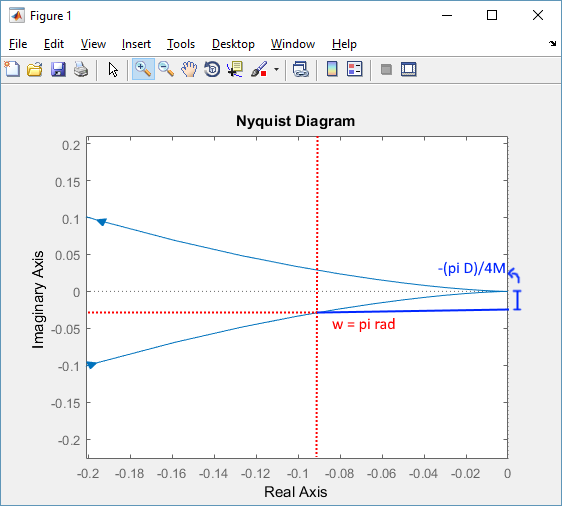
\includegraphics[height=0.4\textheight, keepaspectratio]{nyquist.png}
	\caption{Nyquistkromme met snijpunt waar $\omega = \pi$ rad}
	\label{nyq}
\end{figure}
\begin{figure}[]
	\centering
	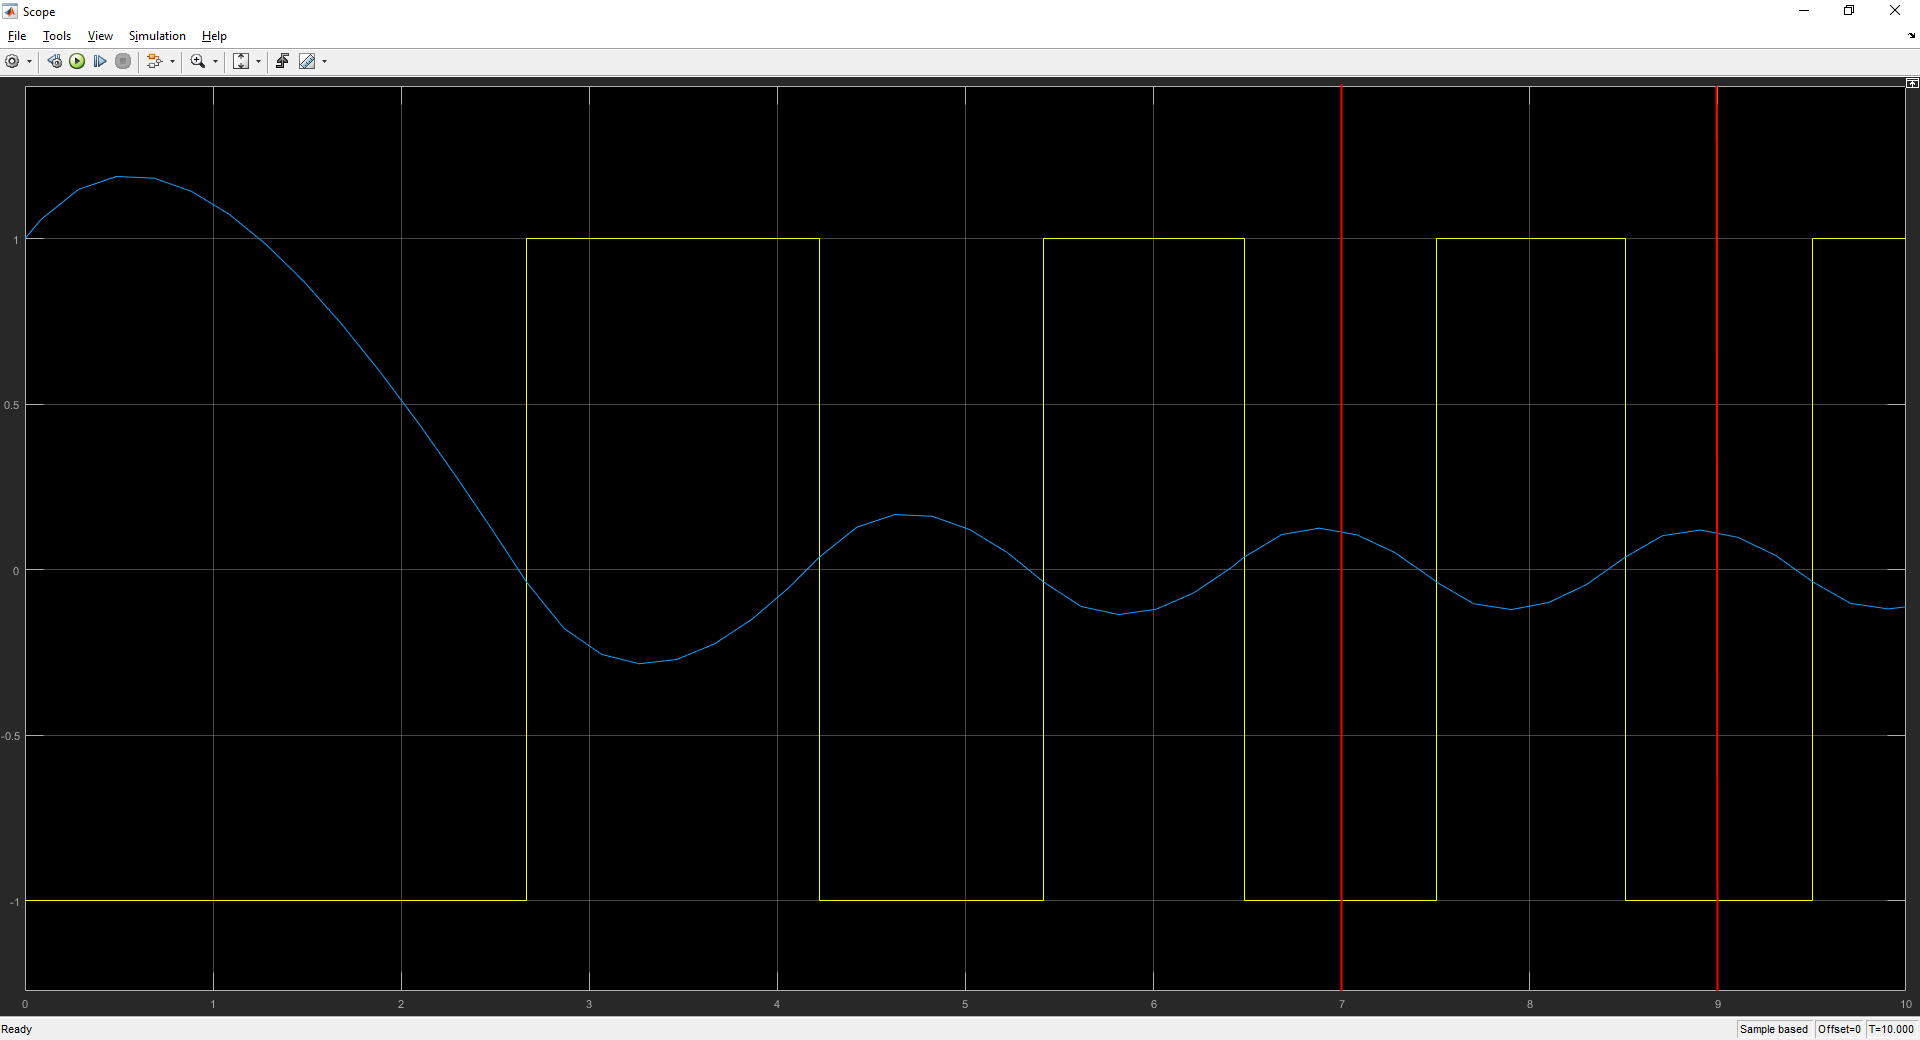
\includegraphics[width=\textwidth, keepaspectratio]{output3.png}
	\caption{Tijdsverloop (10 seconden) met oscillatieduur van 2 seconden}
	\label{output3}
\end{figure}
\clearpage
\subsection{Vergelijking van verschillende simulaties}
Voor het vergelijken van de simulaties werden er 9 curves getekend. Deze grafieken werden gegroepeerd in 3 grafieken met elk 3 curves. Dit met behulp van volgende indeling:
\begin{itemize}
	\item Curves zonder hysteresis
	\item Curves met hysteresis $D = \pm 1$
	\item Curves met hysteresis $D = \pm 0.5$
\end{itemize}
In deze grafieken worden telkens 3 curves getekend met verschillende beginposities. Deze posities zijn de volgende:
\begin{table}[!h]
\centering
	\begin{tabular}{|c|c|c|}
		\hline
		\textbf{kleur} & $\bm{\theta}$ & $\bm{\omega}$ \\
		\hline
		roze & 0.5 & 1.5 \\
		blauw & 1 & 1 \\
		rood & 1 & 1.5 \\
		\hline
	\end{tabular}
\end{table} \\
Hieruit vallen enkele zaken op te merken:
\begin{itemize}
	\item De beginpositie heeft geen invloed op de limietcyclus. Dit zowel bij de simulaties met hysteresis als bij de simulaties zonder. Men spreekt hier van stabiele limietcyclussen.
	\item De hysteresisbreedte blijkt invloed te hebben op de limietcyclus. Dit is ook logisch, gezien de hysteresisbreedte uiteindelijk zorgt voor de amplitude van de limietcyclus. Een lagere hysteresisbreedte zorgt ervoor dat het systeem zich sneller zal willen corrigeren naar de setwaarde, met minder afwijking tot gevolg.
	\item De link tussen de hysteresisbreedte en de oscillatieduur werd eerder verklaard.
\end{itemize}
\clearpage
\begin{figure}
	\centering
	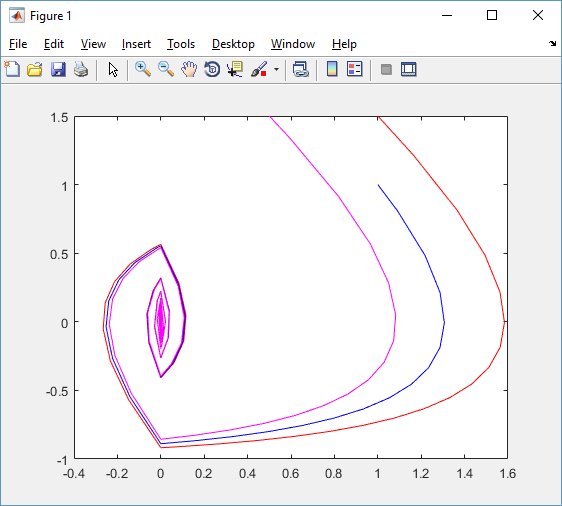
\includegraphics[height=0.4\textheight, keepaspectratio]{xydrienohys.png}
	\caption{$\theta(\omega)$ voor verschillende beginposities (geen hysteresis)}
	\label{xydrienohys}
\end{figure}
\begin{figure}
	\centering
	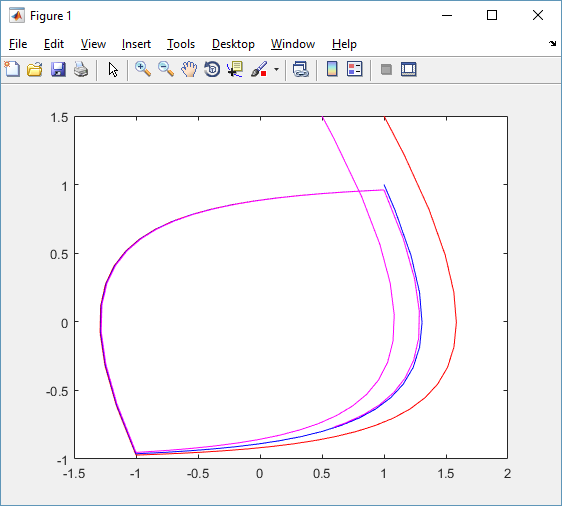
\includegraphics[height=0.4\textheight, keepaspectratio]{xydriehys.png}
	\caption{$\theta(\omega)$ voor verschillende beginposities (met hysteresis $\pm 1$)}
	\label{xydriehys}
\end{figure}
\begin{figure}
	\centering
	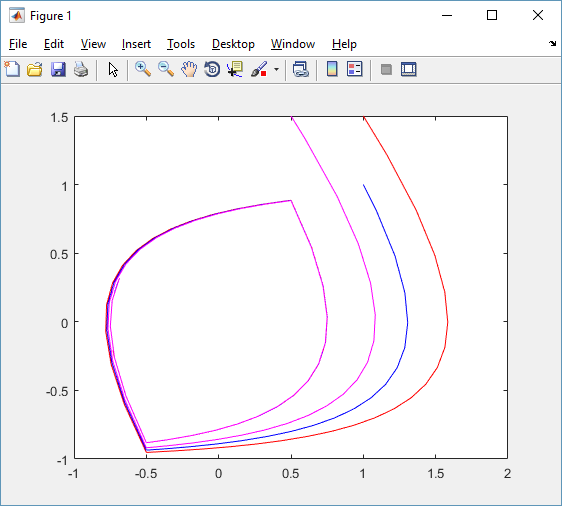
\includegraphics[height=0.4\textheight, keepaspectratio]{xydriehyssmaller.png}
	\caption{$\theta(\omega)$ voor verschillende beginposities (met hysteresis $\pm 0.5$)}
	\label{xydriehys}
\end{figure}
\clearpage
\part{Aan/uit voor temperatuursregeling van een doorstromer}
\setcounter{section}{0}
\section{Introductie}
Voor de aan/uit temperatuursregeling bij een doorstromer wordt gebruik gemaakt van volgende gegevens:
\begin{itemize}
	\item De variatie rond het werkingspunt bedraagt 13.9\degree C
	\item De tijdsconstante van het proces is 1 minuut
	\item De tijdsconstante van de temperatuursensor bedraagt een halve minuut
\end{itemize}
Dit regelschema wordt afgebeeld op figuur \ref{sys2}
\begin{figure}[!h]
	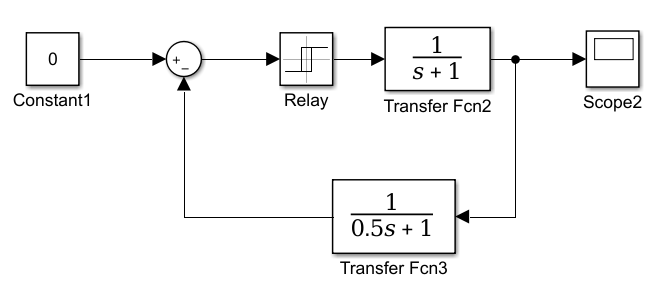
\includegraphics[width=\textwidth ,keepaspectratio]{systeem2.png}
	\centering
	\caption{Temperatuursregeling - regelschema}
	\label{sys2}
\end{figure} \\
Om voor dit schema het fasetraject op te stellen dienen de beginwaarden opnieuw instelbaar te zijn. Dit is mogelijk door de transferfunctie nogmaals op te splitsen in een functie met 2 zuivere integrators. Dit werd gedaan met behulp van het schema uit figuur \ref{schema2}. Er werd een stap aangelegd aan zowel de originele transferfunctie als de zelf geconstrueerde transferfunctie met zuivere integrators. Dit resultaat werd vergeleken in een grafiek alsook in een controlestructuur. 
\begin{figure}[!h]
	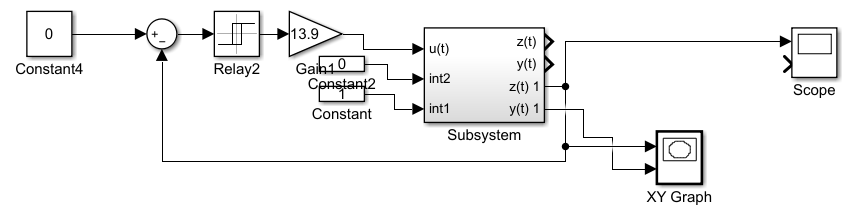
\includegraphics[width=\textwidth ,keepaspectratio]{schemasubsystem.png}
	\centering
	\caption{Equivalent schema temperatuursregeling met controle}
	\label{schema2}
\end{figure} 
\begin{figure}[!h]
	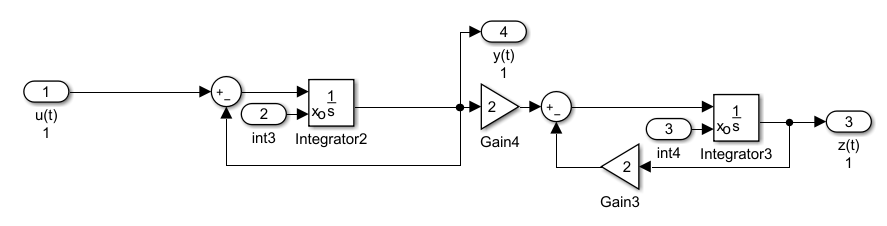
\includegraphics[width=\textwidth ,keepaspectratio]{schemasubsystem2.png}
	\centering
	\caption{Equivalent schema subsystem}
	\label{schema2sub}
\end{figure} 
\section{Simulaties}
\subsection{Tijdsverloop en Fasetraject}
De beginwaarden van de integrators alsook de hysteresisbreedte werd ingesteld naar de gegevens van figuur 29 uit de cursus niet-lineaire regeltechniek. Om het schema uit figuur \ref{schema2sub} te bekomen werd het systeem opgedeeld in 2 eerste orde systemen. Dit leverde de mogelijkheid om $y(t)$ en $z(t)$ eenvoudig de isoleren. De berekening van het subsysteem wordt hieronder gegeven.
\begin{equation}
	\frac{1}{p+1} = \frac{H}{U}
\end{equation}
\begin{equation}
	U = Hp + H
\end{equation}
\begin{equation}
	Hp = U - H
\end{equation}
Dit leverde het linkse deel van figuur \ref{schema2sub}.
\begin{equation}
	\frac{1}{0.5p+1} = \frac{H}{U}
\end{equation}
\begin{equation}
	U = 0.5Hp + H
\end{equation}
\begin{equation}
	Hp = 2U - 2H
\end{equation}
Hierbij stelt $U$ de uitgang van het eerste systeem voor. Deze vergelijking geldt voor het rechtse deel van het subsysteem. De originele uitgangen $z(t)$ en $y(t)$ werden niet gebruikt. De ingangen $int1$ en $int2$ stellen de beginwaarden van de integrators voor. Op deze manier konden deze parameters vanuit de top-level module eenvoudig gewijzigd worden. \\ \\
Figuren \ref{xynohysopgave2} en \ref{xyhysopgave2} stellen de fasetrajecten voor dit systeem voor bij af- en aanwezigheid van hysteresis. Figuren \ref{tijdnohysopgave2} en \ref{tijdhysopgave2} stellen de tijdsresponsen voor. De verklaring voor de fasetrajecten en het tijdsverloop is analoog aan deze van de vorige opgave. Het fundamentele verschil is de aanwezigheid van een driehoekcurve in plaats van een sinuscurve. Dit verschil valt te verklaren doordat er hier gewerkt wordt met een tweede orde systeem.
\begin{figure}[!h]
	\centering
	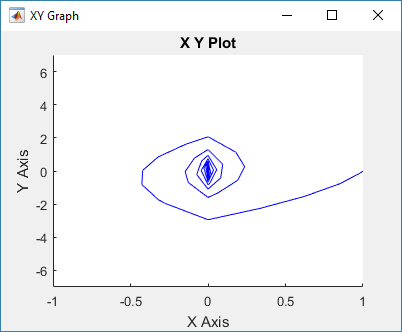
\includegraphics[height=0.4\textheight, keepaspectratio]{xynohysopgave2.png}
	\caption{Fasetraject voor beginparameters (1,0) (zonder hysteresis)}
	\label{xynohysopgave2}
\end{figure}
\begin{figure}[!h]
	\centering
	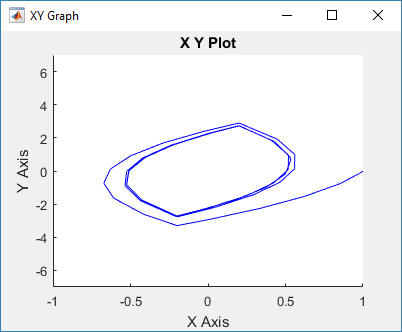
\includegraphics[height=0.4\textheight, keepaspectratio]{xyhysopgave2.png}
	\caption{Fasetraject voor beginparameters (1,0) (hysteresis $\pm 0.2$)}
	\label{xyhysopgave2}
\end{figure}
\begin{figure}[!h]
	\centering
	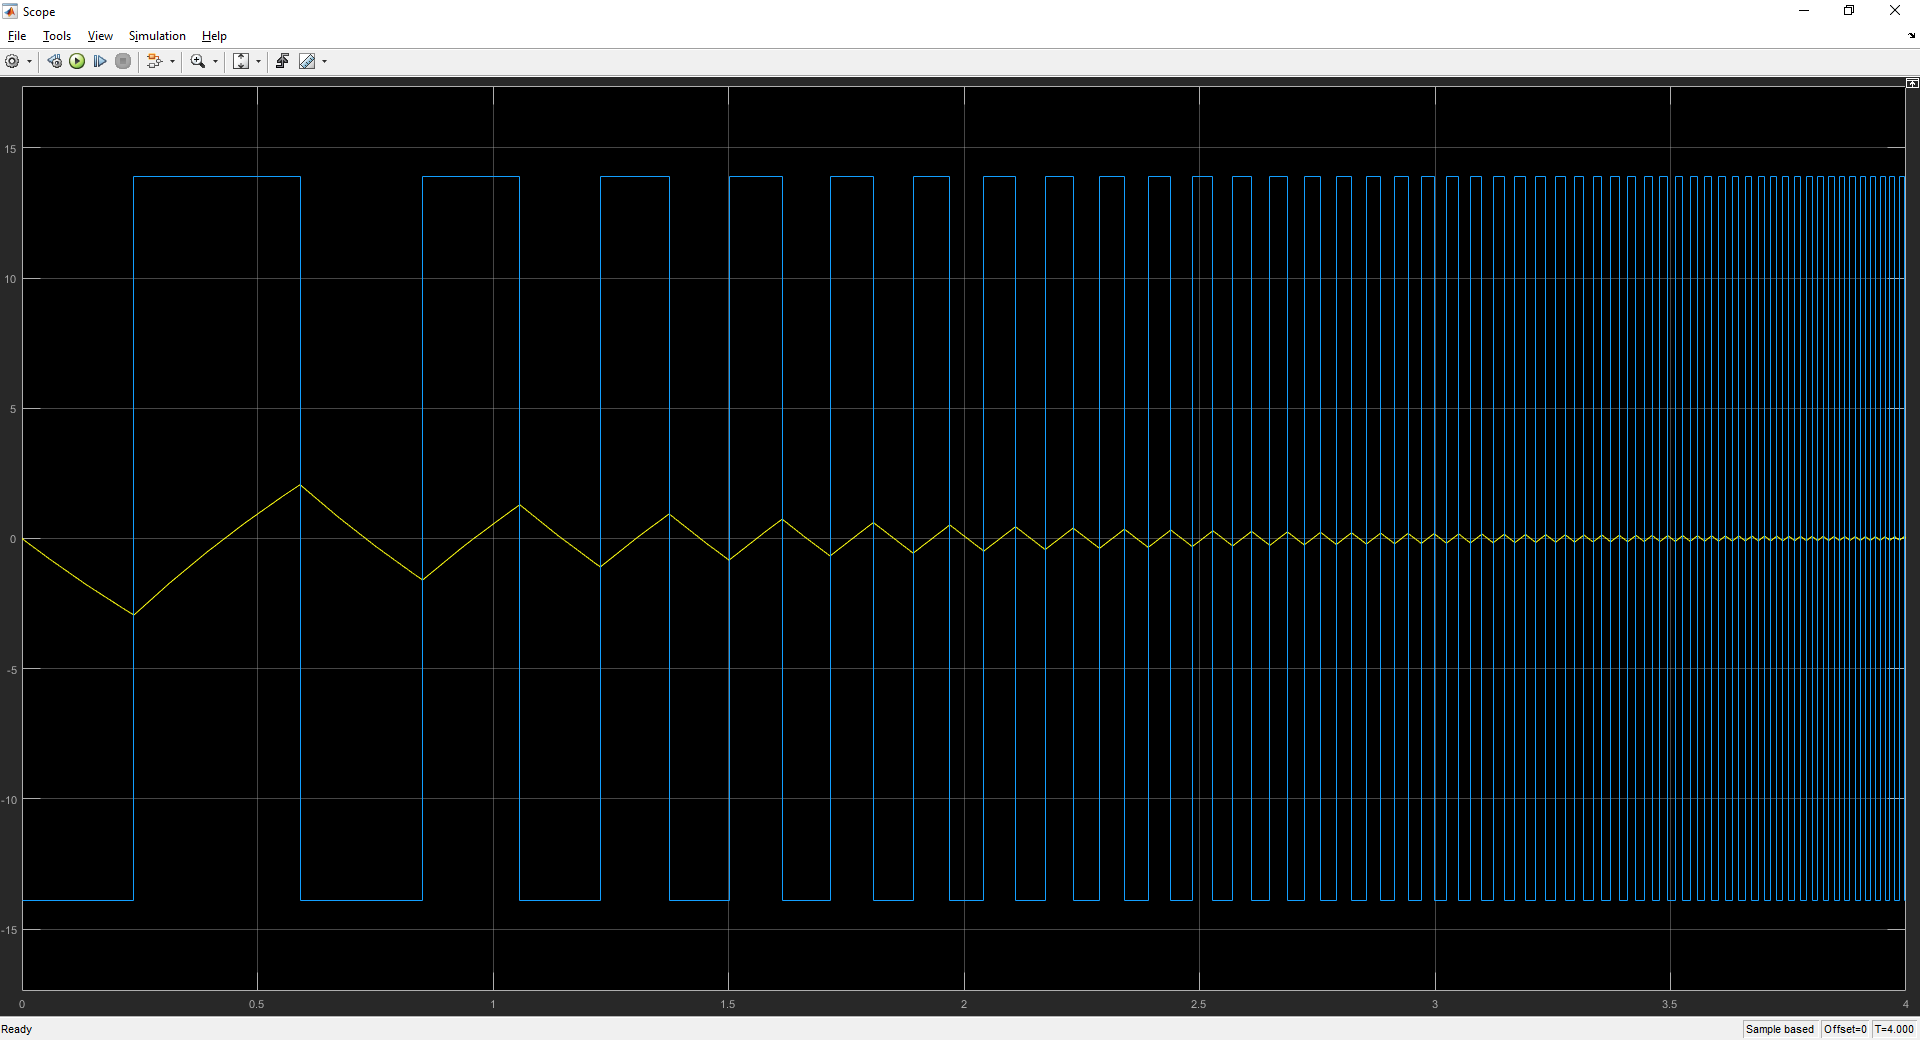
\includegraphics[width=\textwidth, keepaspectratio]{tijdnohysopgave2.png}
	\caption{Tijdsverloop (4 seconden) (zonder hysteresis)}
	\label{tijdnohysopgave2}
\end{figure}
\begin{figure}[!h]
	\centering
	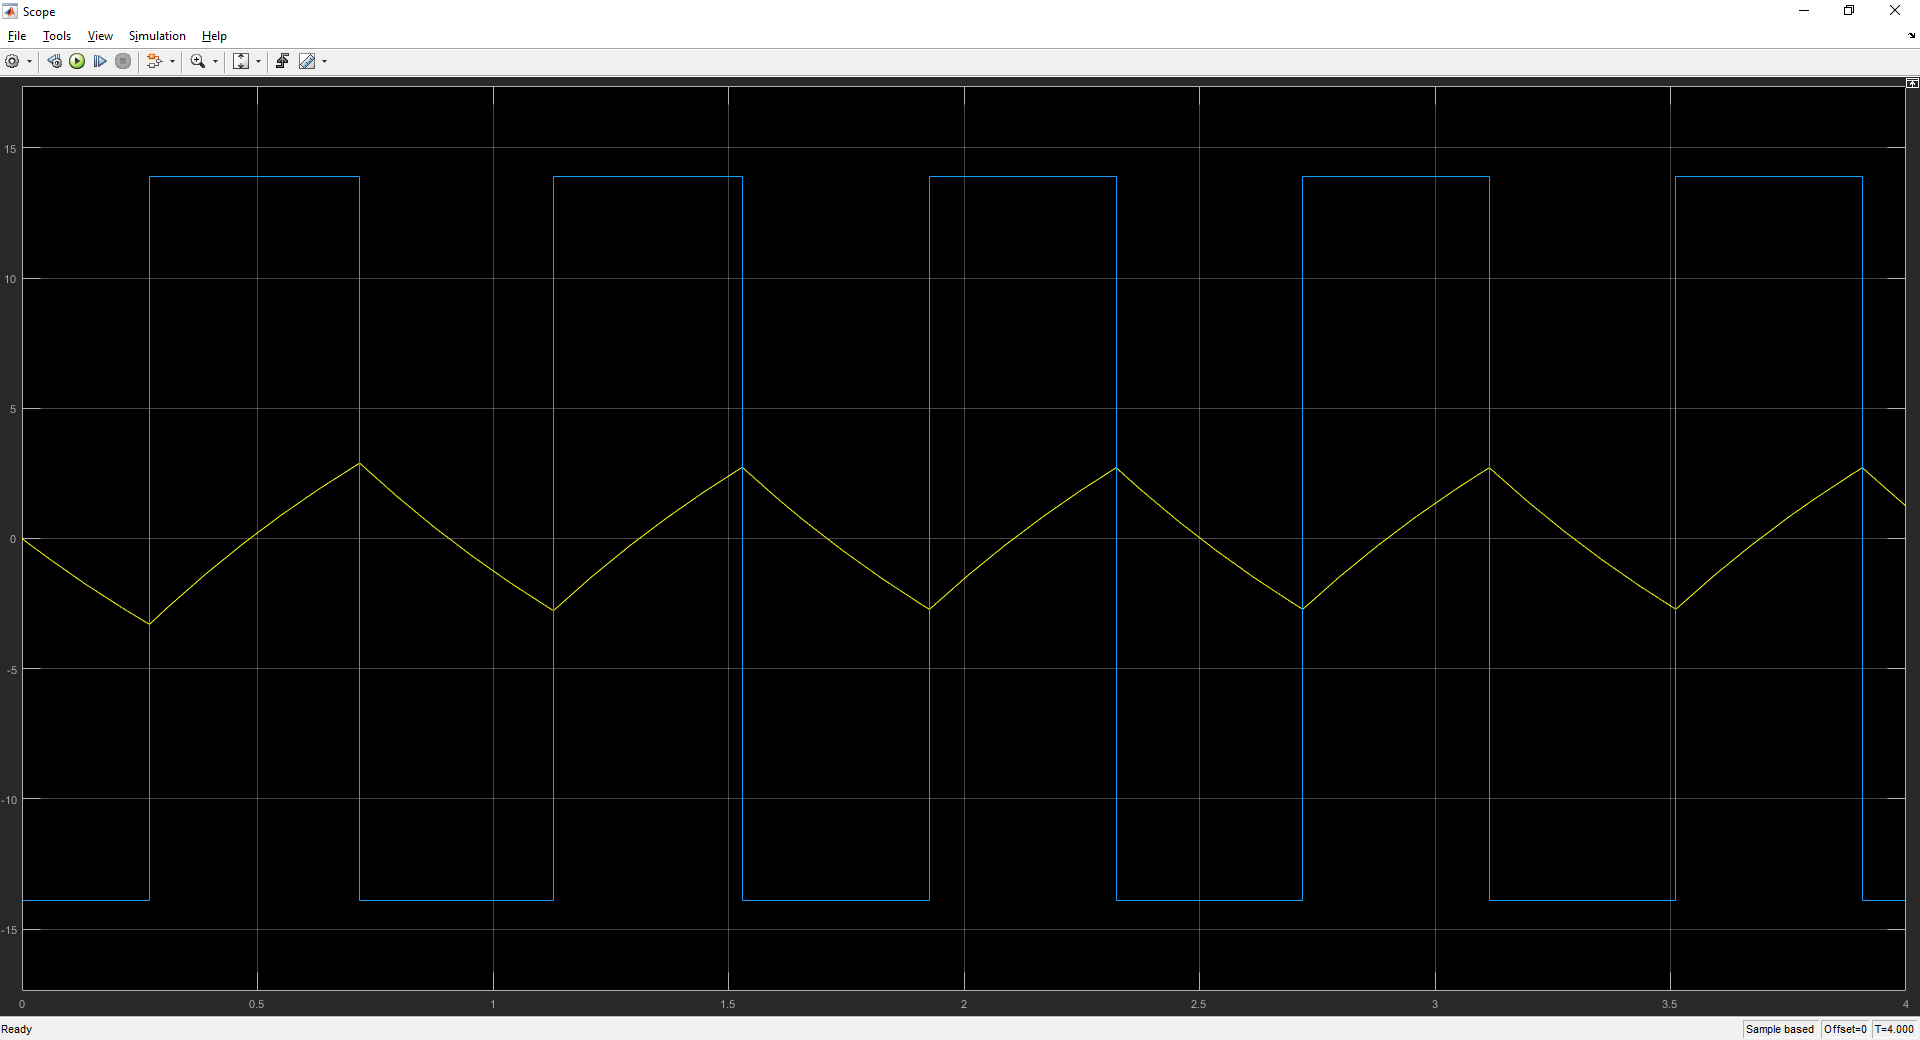
\includegraphics[width=\textwidth, keepaspectratio]{tijdhysopgave2.png}
	\caption{Tijdsverloop (4 seconden) (hysteresis $\pm 0.2$)}
	\label{tijdhysopgave2}
\end{figure}
\clearpage
\subsection{Analyse van de hogere harmonischen}
Om het systeem te analyseren werd er een FFT analyse uitgevoerd op de output $y(t)$. Deze werd gediscretiseerd met behulp van een zero-order-hold operatie. Dit met een samplefrequentie van $f_s = 100Hz$. Het resultaat wordt getoond in figuur \ref{spectrum}. \\ \\
De eerste harmonische is de frequentie waarop het aan/uit element schakelt. Let op dat deze FFT-operatie werd uitgevoerd op de regelkring waarbij het aan/uit element een hysteresisbreedte heeft van $\pm0.2$. Uit figuur \ref{tijdhysopgave2} wordt afgeleid dat de frequentie waarop dit element schakelt ongeveer $\frac{1}{0.8s} = 1.25Hz$. Deze waarde stemt overeen met de frequentie van de eerste piek. \\ \\
Het valt op dat de overige harmonischen veel zwakker zijn dan de eerste harmonische. De derde harmonische heeft slechts een vermogen van $\pm 15 dBm$. De vijfde harmonische zit op ongeveer $3 dBm$. Hieruit kan men besluiten dat de eerste harmonische een redelijk goede benadering geeft voor het niet-lineaire element.
\begin{figure}[!h]
	\centering
	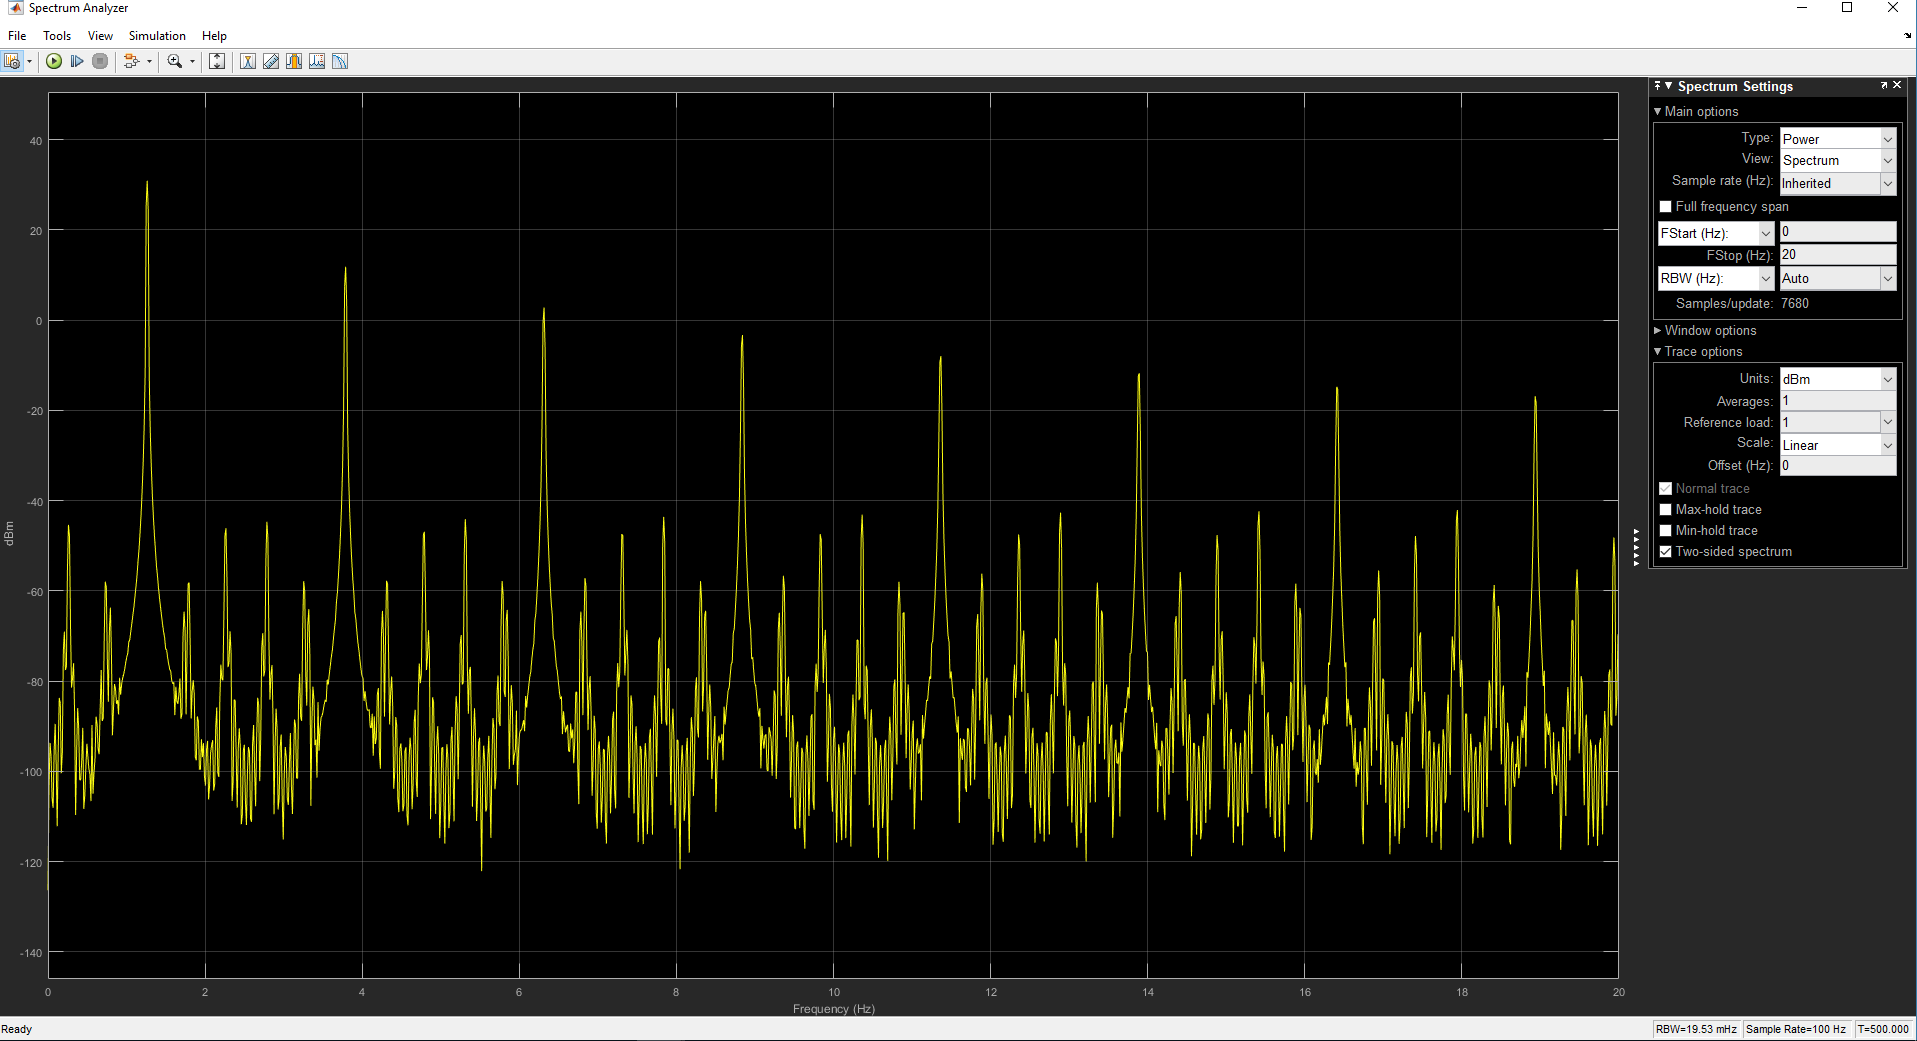
\includegraphics[width=\textwidth, keepaspectratio]{spectrum.png}
	\caption{FFT van $y(t)$ voor frequenties van $0$ tot $20Hz$}
	\label{spectrum}
\end{figure}



\end{document}
